\section{Can Children Learn Pronoun Case from Distributional Patterns}
\subsection{Distributional Patterns in Language Acquisition}
 
The previous sections have reviewed the major theories of children's pronoun case errors. However, none of them seems to be adequate enough to explain why children would make such errors. Furthermore, children rarely make pronoun case errors, that the average error rate is around 1\%. Therefore, instead of asking why children make errors, this paper further pursues how the children acquire pronoun case in the first place. Since cases are used to mark different relationships among arguments in the sentence, the distributional patterns of different cases could be informative enough to differentiate them. For example,  nominative pronouns are more likely to occur before a verb (e.g. `\textit{I} see'), whereas accusative or genitive pronouns rarely appear before a verb (e.g. `*\textit{me/my} see'). However, cases do not have exclusive distributional patterns. Some patterns are shared by more than one case: an accusative pronoun case precede a verb in phrases like `let \textit{him} go' or `help \textit{me} see.' \citep{tomasello2000}. Are children able to learn pronoun case from distributional patterns in the face of ambiguity?

Distributional information can be effective in grammatical categorization tasks. \citet{redington1998distributional} demonstrated that the context of a target word, including the previous words and following words, can be used to cluster the target word into different grammatical categories. Their model achieved high accuracy in categorization in general; however, for words that appear in less frequent contexts, accuracy suffered.  \citet{mintz2003frequent} proposed that frequent local trigram frames consisting of one word before the target word and one word following it (an \texttt{aXb} frame, where \texttt{X} is the target word) contain enough information for grammatical categorization. For example, in the frame `to \texttt{X} to', \texttt{X} is likely to be a verb, e.g. `to go to'. Mintz examined the 45 most frequent \texttt{aXb} frames in parents' input and showed that the accuracy for \texttt{X}'s grammatical categorization was over 0.90. However, only a small portion of words appear in the frequent \texttt{aXb} frames. In order to categorize more words, \citet{clair2010learning} separated the \texttt{aXb} frame into two bigram frames: \texttt{aX + Xb}. They suggested that instead of learning the co-occurring frame `\texttt{a\_b}' as a whole unit, it is more efficient to treat it as two flexible bigrams `\texttt{a\_}' and `\textt{\_b}' which are more useful in learning.  They trained feedforward neural networks on 100,000 samples of the \texttt{aXb} frame and the \texttt{aX + Xb} frame had better categorization accuracy (0.73) than the \texttt{aXb} frame (0.53). Grammatical cases are similar to grammatical categories in that both reflect certain syntactic features of the word. In the next subsection, models using \texttt{aXb} and \texttt{aX + Xb} frames are trained to predict the pronoun case of \texttt{X}  The purpose of this section is not to provide a model to explain children's grammatical case acquisition, but to examine if the distributional patterns in parents' input are informative enough to distinguish pronoun cases. The results do not indicate whether children acquire pronoun case from parents' input but suggest a possible source from which children could learn pronoun case.

\subsection{Methods}
\label{sec:methods}
\subsubsection{Corpus Summary}
Following \citet{mintz2003frequent} and \citet{clair2010learning}, the same six corpora of child-directed speech from CHILDES \cite{macwhinney2014childes} were used: Anne and Aran \cite{theakston2001}, Eve \cite{brown1973first}, Naomi \cite{sachs1983talking}, Nina \cite{suppes1974semantics}, Peter \cite{bloom1974imitation}. Utterances in the files where the child is younger than 2;6 years old were analyzed. The pronouns were extracted with the part-of-speech tags assigned by the MOR parser \cite{macwhinney2012morphosyntactic} in CHILDES: \texttt{pro:sub} for nominative pronouns, \texttt{pro:obj} for accusative pronouns and \texttt{det:poss} for genitive pronouns. Case-ambiguous pronouns `you' and `it' were excluded from the study since they were tagged as \texttt{pro:per} in all argument positions. The pronoun `her' was included since it was tagged as \texttt{pro:obj} for its accusative use and \texttt{det:poss} for its genitive use. Each pronoun was extracted with its \texttt{aXb} context. Table \ref{tab:le1}summarizes the number of tokens of all pronouns and each case, and the number of types for \texttt{aX}, \texttt{Xb} and \texttt{aXb}. Figure \ref{fig:1} shows the token frequencies of the pronouns produced by the children's parents.

\FloatBarrier
\begin{table}[!h]
\centering
\caption{Token counts of three pronoun cases and type counts of three context frames}
\label{tab:le1}
\begin{tabular}{llllllll}
\toprule
 & \textbf{NOM} & \textbf{ACC} & \textbf{GEN} & \textbf{Pronoun Tokens} & \textbf{aX types} & \textbf{Xb types} & \textbf{aXb types} \\ \hline
Aran & 4518 & 1014 & 1454 & 6986 & 445 & 927 & 2489 \\
Anne & 4343 & 1080 & 1392 & 6815 & 428 & 707 & 2308 \\
Eve & 1292 & 479 & 1029 & 2800 & 278 & 500 & 1364 \\
Naomi & 599 & 249 & 503 & 1352 & 224 & 364 & 806 \\
Nina & 3490 & 1195 & 1571 & 6256 & 400 & 747 & 2376 \\
Peter & 339 & 135 & 207 & 681 & 187 & 250 & 475 \\
\textbf{Total} & 14581 & 4152 & 6156 & 24889 & 898 & 1672 & 7355 \\ 
\toprule
\end{tabular}
\end{table}
\FloatBarrier

\FloatBarrier
\begin{figure}[!h]
    \centering
    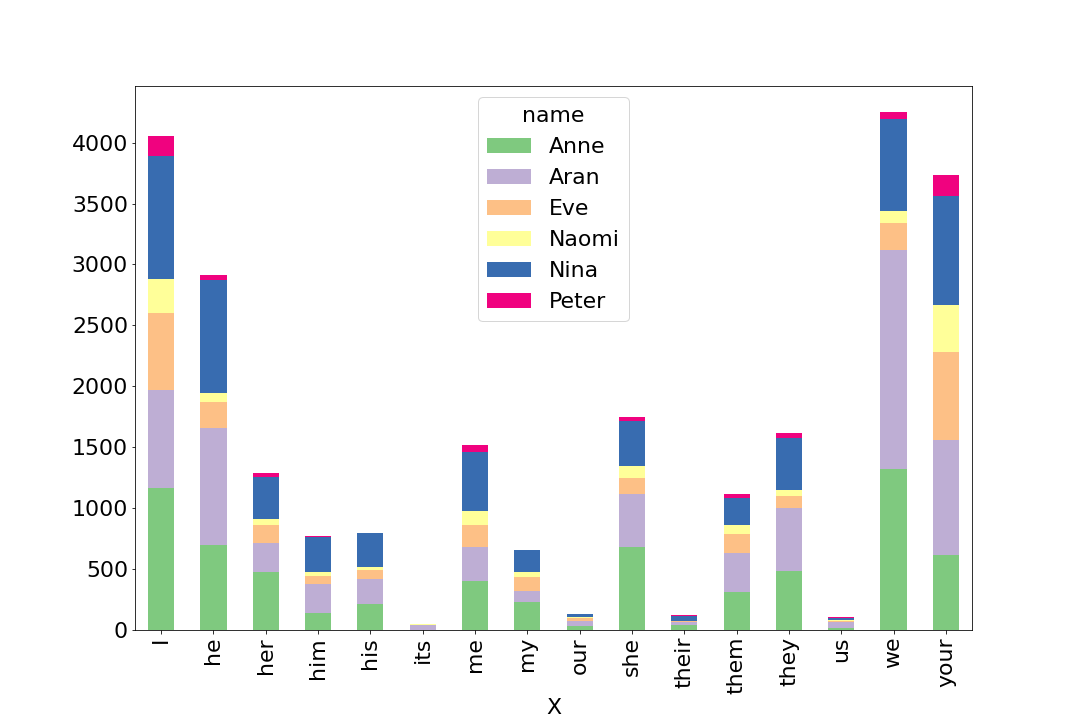
\includegraphics[scale=0.45]{graph/Stackedbar.png}
    \caption{Pronoun tokens by the parents of six children}
    \label{fig:1}
\end{figure}
\FloatBarrier



\subsubsection{Model Architecture}
Supervised learning with a feedforward connectionist model was used to compare the accuracy of the \texttt{aXb} model and the \texttt{aX + Xb} model. For the \texttt{aXb} model, the input consisted of one one-hot vector, representing `\texttt{a\_b}'. For the \texttt{aX + Xb} model, the input consisted of two one-hot vectors, representing `\texttt{a\_}' and `\texttt{\_b}' respectively. The two models are shown in Figure \ref{fig:2} and Figure \ref{fig:3}, with `let me do' as an example. For the \texttt{aXb} model, the input unit represents `let\_do'. For the \texttt{aX + Xb} model, one input represents `let\_' and the other input represents `\_do'.  The connectionist model used the following parameters: (1) number of hidden units was set to 200 and initialized randomly for each model; (2) the non-linearity was relu.  
\begin{figure}[ht]
   \centering
    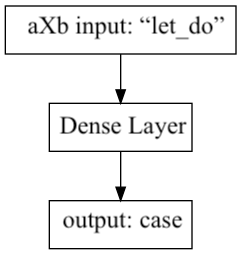
\includegraphics[scale = 0.4]{graph/aXb.png}
    \caption{The architecture of \texttt{aXb} model}
    \label{fig:2}
    \centering
    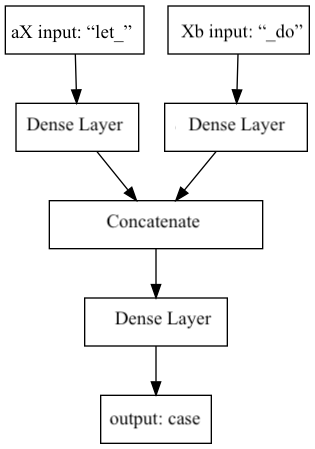
\includegraphics[scale = 0.5]{graph/aX+Xb.png}
    \caption{The architecture of \texttt{aX + Xb} model}
    \label{fig:3}
\end{figure}
\subsubsection{Evaluation}
The classification accuracy for each case was used to compare the \texttt{aXb} model and \texttt{aX + Xb} models. In addition, following \citet{clair2010learning} asymmetric lambda value \citet{goodman1979measures} was also reported to evaluate the association among the classification of grammatical cases. Lambda is defined as the proportional reduction in prediction error. It provides insight into the extent to which the model's prediction is based on the actual category. Lambda is in the range of [0,1], where 0 indicates there is no association between predicted and actual categories, and 1 indicates a perfect association. For example, if the model categorizes all frames as nominative cases simply because that is the most frequent case, then the accuracy will be 0.586 (14581/24889), but the lambda will be 0. 
\subsubsection{Training and Testing}
The classification accuracy of models were measure and compared by applying 10-fold cross validation on the union of the six children's corpora. The \texttt{aXb} model and \texttt{aX + Xb} model were trained using the same 10-fold cross-validation split. All the frames were used for both training and testing. 

Adam optimization algorithm was used to minimize the mean squared error (MSE) loss function over the training data. The model was trained on a maximum of 100 epochs with a batch size of 32. Early stopping methods were applied to stop the training when the accuracy did not change in 10 consecutive training rounds. 


\subsection{Experiment 1: Models \texttt{aXb} vs \texttt{aX + Xb} in Categorizing Grammatical Cases}
All models were trained and evaluated following the steps in \ref{sec:methods}. Following \cite{clair2010learning}, the training of each model was split into a token-training phase and a type-training phase. In the token-training phase, the models were trained on all 24889 pronoun patterns. In the type-training phase, the models were trained only on 7355 tokens of unique \texttt{aXb} types. Tables \ref{tabletable:3} and \ref{tabletable:4} show the overall classification accuracies and lambda scores of \texttt{aXb} and \texttt{aX + Xb} on each child's corpus. Both models achieved very high accuracy with 24889 tokens. In addition, the lambda scores showed that almost perfect associations, suggesting that the \texttt{aXb} and \texttt{aX + Xb} models are very effective in predicting the correct grammatical case. Figures \ref{fig:heatmap1} and \ref{fig:heatmap2} show the heatmaps of the classification results. All three cases are classified with high accuracy. The heatmaps also indicate that the two models make different classification errors. For example, for genitive case, the \texttt{aX + Xb} model is more likely to miscategorize it as an accusative case whereas the \texttt{aXb} model is more likely to label it as a nominative case.  
\FloatBarrier
\begin{table}[!h]
\centering
\caption{Results of training on 24889 total tokens}
\label{tabletable:3}
\begin{tabular}{lllll}
\hline
 & \multicolumn{2}{l}{\textbf{\texttt{aX + Xb}}} & \multicolumn{2}{l}{\textbf{
\texttt{aXb}}} \\ \hline
 & \textbf{Accuracy} & \textbf{$\lambda$} & \textbf{Accuracy} & \textbf{$\lambda$} \\ \hline
Aran & 0.984 & 0.956 & 0.962 & 0.894 \\
Anne & 0.984 & 0.957 & 0.962 & 0.897 \\
Eve & 0.979 & 0.961 & 0.960 & 0.928 \\
Naomi & 0.983 & 0.969 & 0.951 & 0.914 \\
Nina & 0.987 & 0.970 & 0.951 & 0.911 \\
Peter & 0.982 & 0.965 & 0.954 & 0.913 \\
\textbf{Total} & \textbf{0.984} & \textbf{0.962} & \textbf{0.960} & \textbf{0.907} \\ \hline
\end{tabular}
\end{table}
\FloatBarrier
\FloatBarrier
\begin{table}[!h]
\centering
\caption{Results of Training on 7355 tokens of unique types}
\label{tabletable:4}
\begin{tabular}{lllll}
\hline
 & \multicolumn{2}{l}{\textbf{\texttt{aX + Xb}}} & \multicolumn{2}{l}{\textbf{\texttt{aXb}}} \\ \hline
 & \textbf{Accuracy} & \textbf{$\lambda$} & \textbf{Accuracy} & \textbf{$\lambda$} \\ \hline
Aran & 0.968 & 0.940 & 0.849 & 0.631 \\
Anne & 0.963 & 0.936 & 0.841 & 0.639 \\
Eve & 0.968 & 0.931 & 0.872 & 0.648 \\
Naomi & 0.953 & 0.902 & 0.878 & 0.708 \\
Nina & 0.974 & 0.952 & 0.834 & 0.600 \\
Peter & 0.963 & 0.927 & 0.827 & 0.619 \\
\textbf{Total} & \textbf{0.967} & \textbf{0.939} & \textbf{0.847} & \textbf{0.631} \\ \hline
\end{tabular}
\end{table}
\FloatBarrier

\FloatBarrier
\begin{figure}[!h]
    \centering
    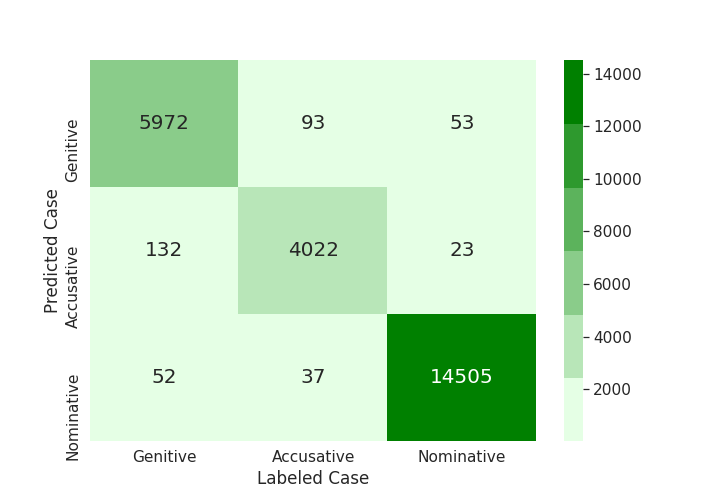
\includegraphics[scale = .45]{graph/aXXbheatmap24889.png}
    \caption{Heatmap of each case's classification in \texttt{aX + Xb} model of 24889 total tokens}
    \label{fig:heatmap1}
    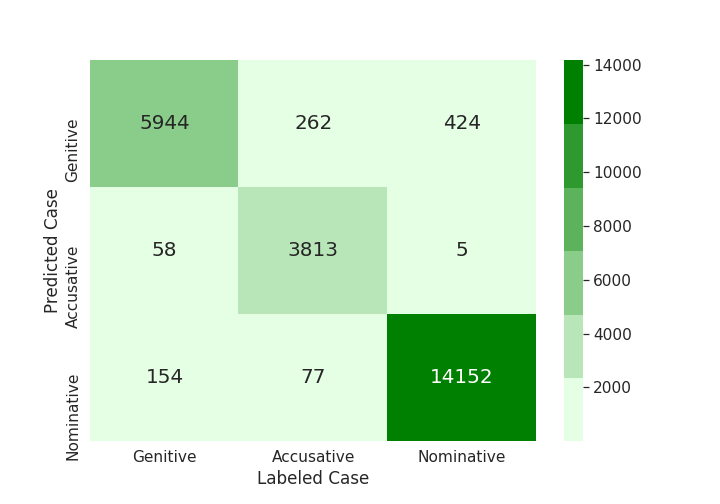
\includegraphics[scale =.45]{graph/aXbheatmap24889.png}
    \caption{Heatmap of each case's classification in \texttt{aXb} model of 24889 total tokens}
    \label{fig:heatmap2}
\end{figure}
\FloatBarrier

When the sample size drops to 7355 tokens, the accuracies and the lambda scores also change for both models. The performance of \texttt{aX + Xb} is not heavily affected by a smaller sample size: the accuracy changes from 0.984 to 0.967 and the lambda score changes from 0.962 to 0.939. In contrast, the \texttt{aXb} model shows a large decline in the accuracy and the lambda score when the sample size drops: the accuracy falls to 0.847 and the lambda score drops to 0.631. Thus, \texttt{aX + Xb} not only has higher accuracy, but also is less vulnerable to small sample size. Figures \ref{fig:heatmap3} and \ref{fig:heatmap4} are the classification heatmaps of each case.

\FloatBarrier
\begin{figure}[!h]
  \centering
    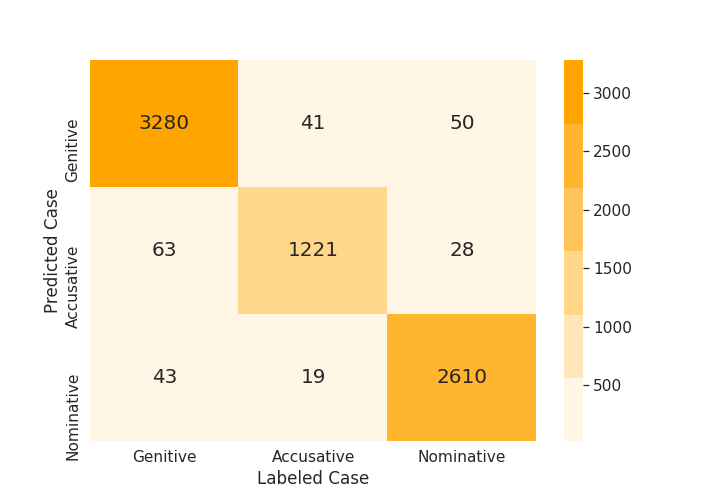
\includegraphics[scale = 0.45]{graph/aXXbheatmap7355.png}
    \caption{Heatmap of each case's classification in \texttt{aX + Xb} model of 7355 tokens of unique types}
    \label{fig:heatmap3}
    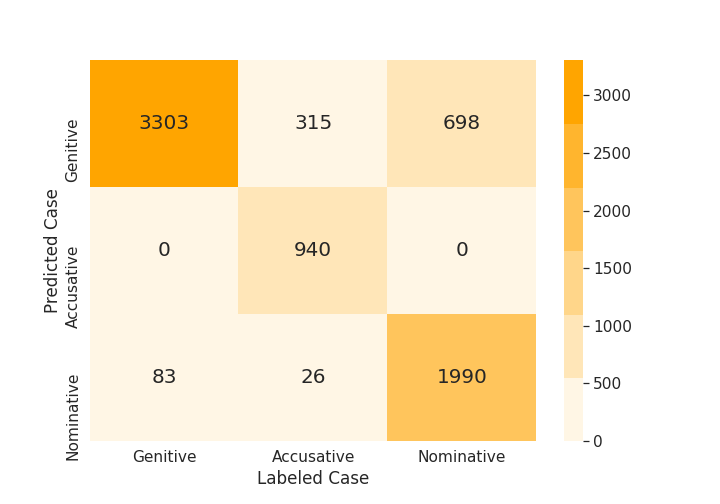
\includegraphics[scale = .45]{graph/aXbheatmap7355.png}
    \caption{Heatmap of each case's classification in \texttt{aXb} model of 7355 tokens of unique types}
    \label{fig:heatmap4} 
\end{figure}
\FloatBarrier

The classification accuracies of each pronoun for each child's input were also plotted, which can be found in Figures \ref{fig:11} - \ref{fig:14}.
\FloatBarrier
\begin{figure}[!h]
\centering
    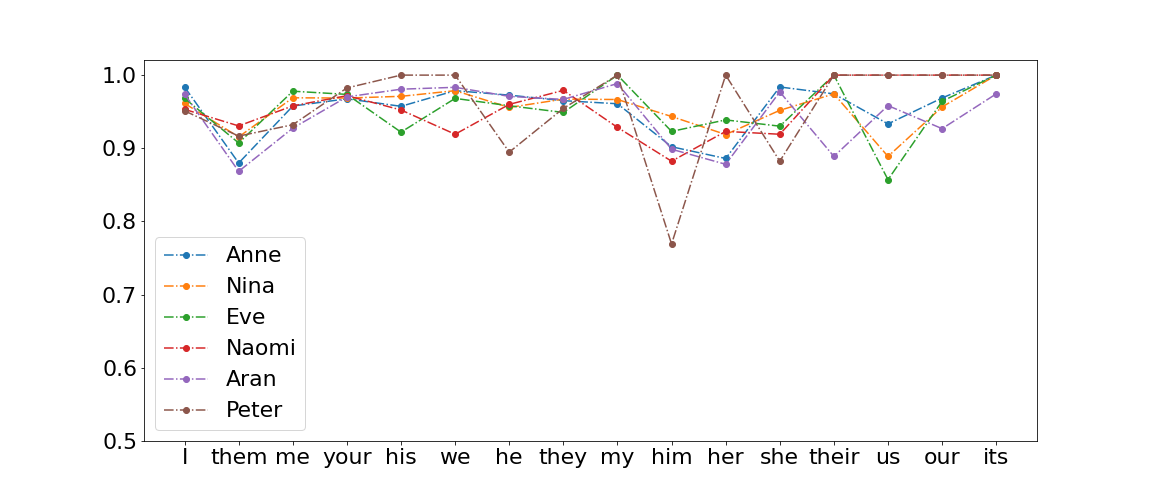
\includegraphics[scale = 0.3]{graph/AXbdots.png}
    \caption{\footnotesize{\texttt{aXb} model accuracy with 24889 total tokens}}
    \label{fig:11}
    %\vspace{-em}
    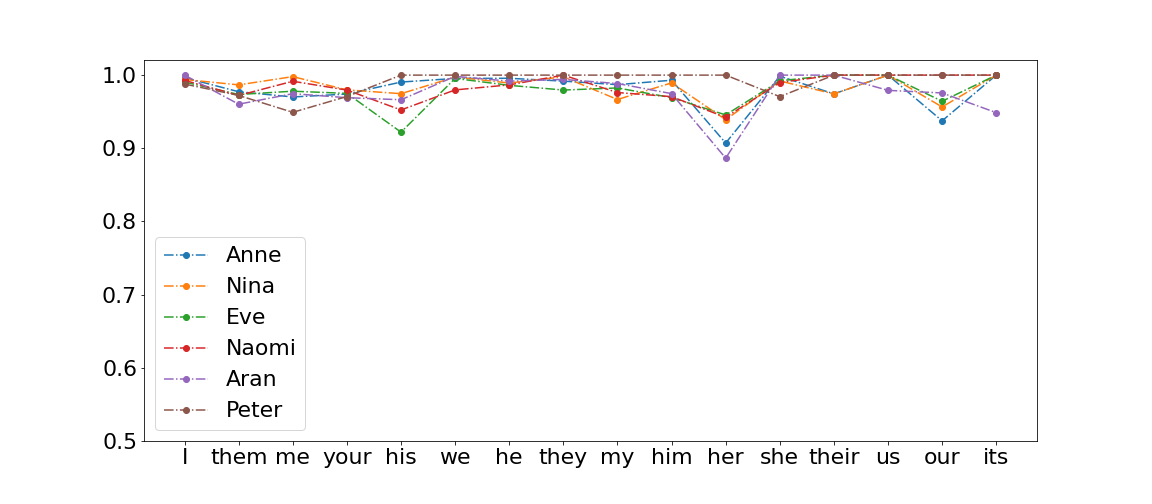
\includegraphics[scale = 0.3]{graph/AXXbdots.png}
    \caption{\footnotesize\texttt{aX+Xb} model accuracy with 24889 total tokens}
     %\vspace{-2em}
    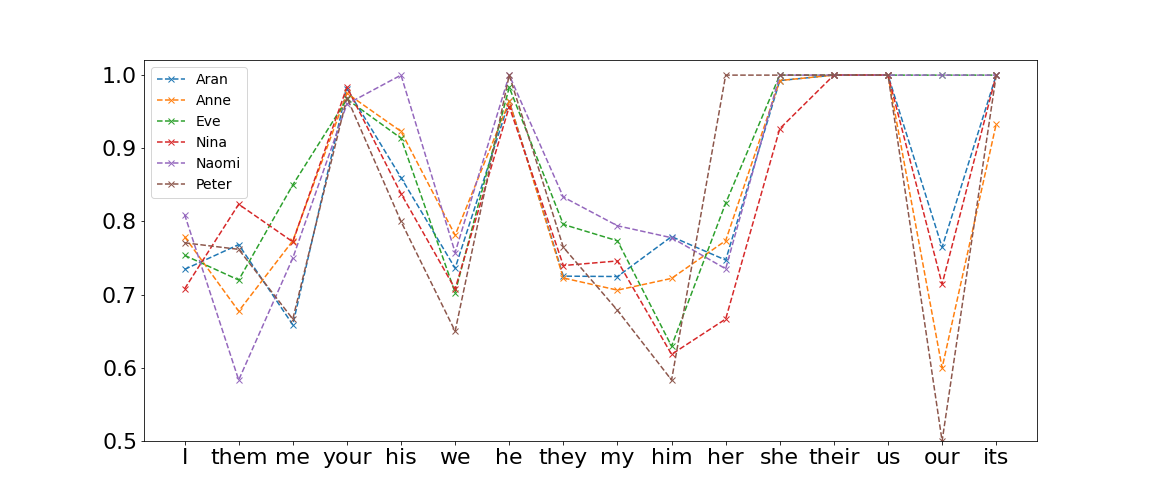
\includegraphics[scale = 0.3]{graph/AXbdots7355.png}
    \caption{\footnotesize\texttt{aXb} model accuracy with 7355 tokens of unique types}
     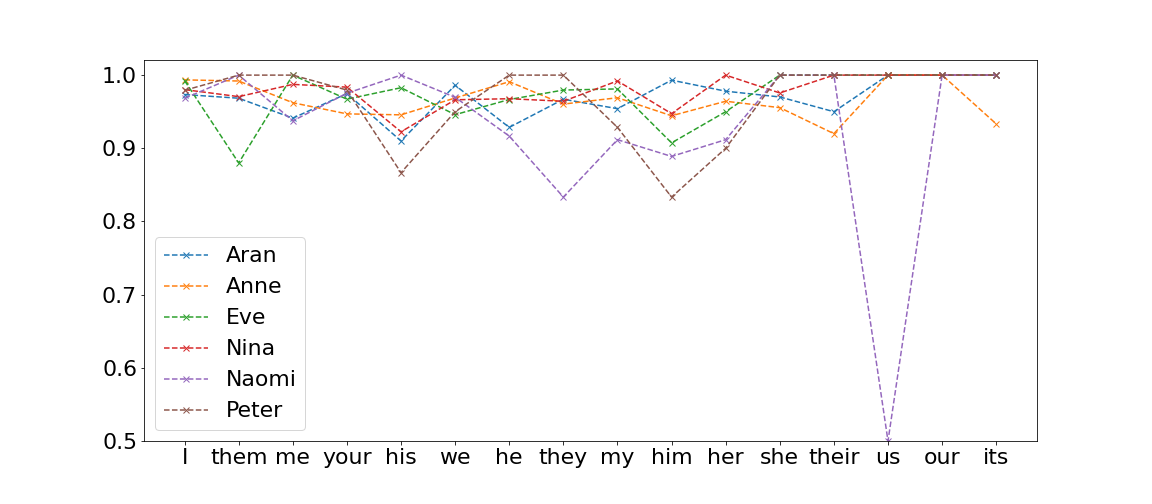
\includegraphics[scale = 0.3]{graph/AXXbdots7355.png}
    \caption{\texttt{aX + Xb} model accuracy for each pronoun with 7355 tokens of unique types}
    \label{fig:14}
\end{figure}
\FloatBarrier

\subsection{Experiment 2: Predicting the Pronoun Using \texttt{aX + Xb} Model with Person, Gender, Number Information}
\label{sec:Experiment2}

Since the \texttt{aX + Xb} model achieved high accuracy in grammatical case classification, the next question being asked is that if the pronoun can be effectively predicted when person, gender and number information are given in training. In the second experiment, the person, gender, and number information for each pronoun (e.g. `he' would be coded as third-person, masculine and singular) were coded and added as an additional input to the \texttt{aX + Xb} model. The model was trained on the same 24889 total tokens and 7355 tokens of unique types as in Experiment 1, and used the same 10-fold cross-validation splits. 

Table \ref{tablepp:4} shows the results. With gender, person and number as additional input, the \texttt{aX + Xb} model can predict the pronoun at an accuracy of 0.994 with 24889 total tokens and 0.982 with 7355 tokens of unique types. In addition, the lambda scores indicate an almost perfect association. Given additional information on person, gender, and number, the \texttt{aX + Xb} model is extremely effective in predicting the pronoun. 

\FloatBarrier
\begin{table}[!h]
\centering
\caption{Results of \texttt{aX + Xb} model Predicting Pronoun on 24889 and 7355 tokens with gender, number, person information }
\label{tablepp:4}
\begin{tabular}{lllll}
\toprule
 & \multicolumn{2}{l}{\textbf{24889 tokens}} & \multicolumn{2}{l}{\textbf{7355 types}} \\ \hline
 & \textbf{Accuracy} & \textbf{$\lambda$} & \textbf{Accuracy} & \textbf{$\lambda$} \\ \hline
Aran & 0.994 & 0.992 & 0.980 & 0.971 \\
Anne & 0.994 & 0.992 & 0.980 & 0.976 \\
Eve & 0.993 & 0.990 & 0.983 & 0.972 \\
Naomi & 0.993 & 0.995 & 0.980 & 0.967 \\
Nina & 0.996 & 0.994 & 0.987 & 0.982 \\
Peter & 1.000 & 1.000 & 0.983 & 0.975 \\
\textbf{Total} & \textbf{0.994} & \textbf{0.993} & \textbf{0.982} & \textbf{0.975} \\ \toprule
\end{tabular}
\end{table}
\FloatBarrier


Figures \ref{fig:heatmap5} and \ref{fig:heatmap6} show the classification results for each pronoun. The classification errors on each pronoun are usually case errors (e.g. `I' mislabeled as 'me' or 'my'). There are few errors on the gender (e.g. `he' mislabeled as `she') and almost no errors on number and person. Each child's pronoun accuracy in shown in Figures \ref{figg:15} and \ref{figg:16}. 
\FloatBarrier
\begin{figure}[!h]
    \centering
    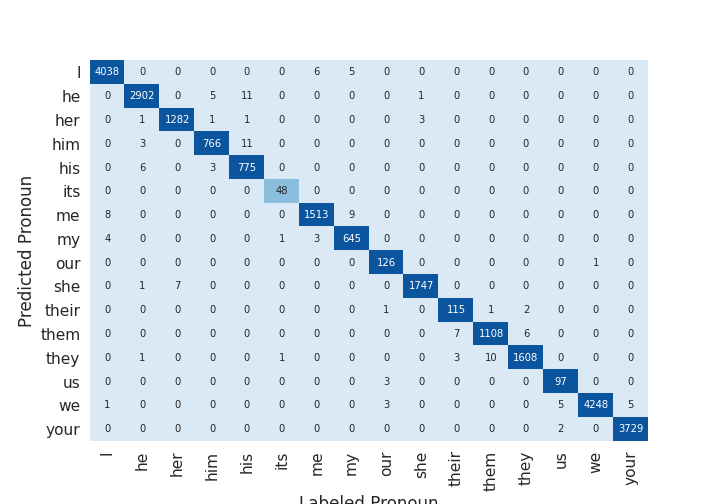
\includegraphics[scale = 0.55]{graph/aXbheatmap24889pronoun.png}
    \caption{Heatmap of pronoun classification results on 24889 total tokens}
    \label{fig:heatmap5}
    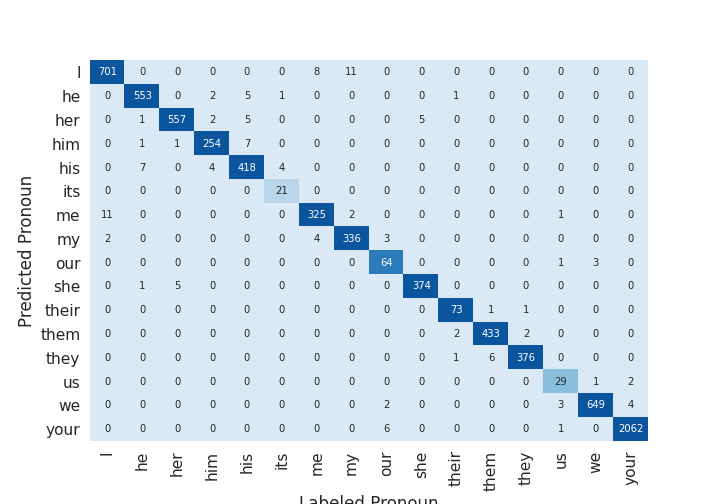
\includegraphics[scale = 0.55]{graph/aXbheatmap7355pronoun.png}
    \caption{Heatmap of pronoun classification results on 7355 tokens of unique types}
    \label{fig:heatmap6}
\end{figure}
\FloatBarrier

\FloatBarrier
\begin{figure}[!h]
    \centering
   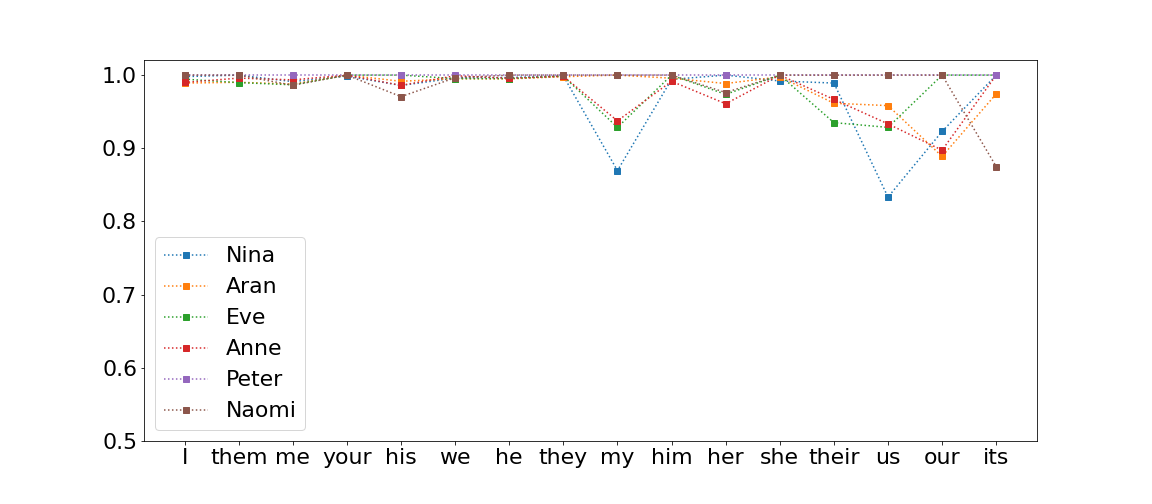
\includegraphics[scale = 0.45]{graph/aXXbpron24889.png}
    \caption{Accuracies of \texttt{aX + Xb} model with person, gender, number information for each pronoun with 24889 total tokens}
    \label{figg:15}
    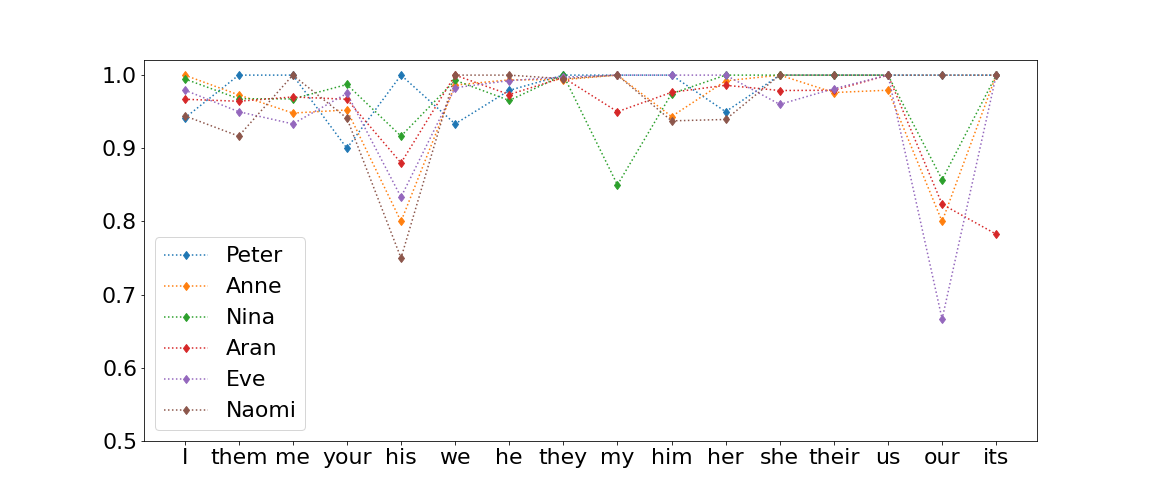
\includegraphics[scale = 0.45]{graph/aXXbpron7355.png}
\caption{Accuracies of \texttt{aX + Xb} model with person, gender, number information for each pronoun with 7355 tokens of unique types}
\label{figg:16}
\end{figure}
\FloatBarrier

\subsection{Experiment 3: Corpus Analysis of Children's Pronoun Case Error Patterns}
Experiments 1 and 2 have show that distributional patterns are extremely effective in pronoun case categorization, suggesting that parents' input is informative for pronoun case learning. In experiment 3, children's pronoun learning were examined. Each child's pronoun case errors and total tokens of pronouns were counted. Table \ref{table:5758} shows the accuracy for each child's pronoun case use. Most children have very high accuracy in their pronoun case uses, except for Nina, whose accuracy is 0.926. The overall pronoun case accuracy for all 6 children is 0.97, which is similar to the results of the \texttt{aX + Xb} model (0.967 for unique types and 0.984 for total tokens ). 
\FloatBarrier
\begin{table}[!h]
\centering
\caption{Results of each child's pronoun case errors and accuracy}
\label{table:5758}
\begin{tabular}{lllll}
\hline
 & \textbf{Errors} & \textbf{Total Pronouns} & \textbf{Accuracy} \\ \hline
Anne  & 57 & 5009 & 0.989 \\
Aran & 25 & 8450 & 0.997 \\
Peter& 115 & 4077 & 0.971 \\
Eve  & 49 & 2685 & 0.982 \\
Naomi  & 64 & 3249 & 0.980 \\
Nina  & 633 & 8609 & 0.926 \\
\textbf{Total} & \textbf{943} & \textbf{32079} & \textbf{0.970} \\ \hline
\end{tabular}
\end{table}
\FloatBarrier

Figure \ref{fig:heatmapchi} shows children's errors on pronoun cases. Children's errors are different from the classification models' errors. For example, the children never mistreated a genitive pronoun or a nominative pronoun as an accusative pronoun. 

\FloatBarrier
\begin{figure}[!h]
    \centering
    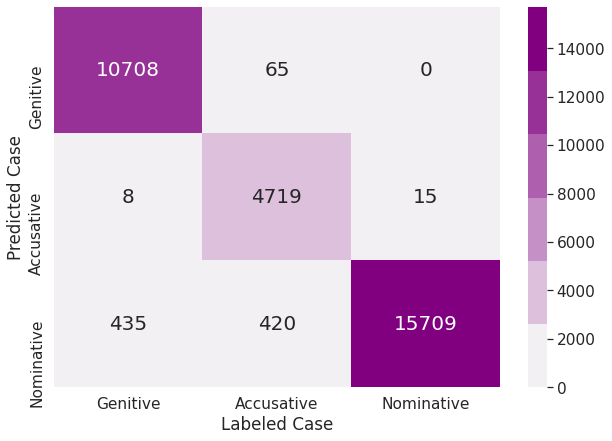
\includegraphics[scale = 0.45]{graph/chiheatmap.png}
    \caption{Heatmap of pronoun case uses by children}
    \label{fig:heatmapchi}
\end{figure}
\FloatBarrier

In addition, the model also made errors that are rarely reported in the literature of children's pronoun errors, such as gender error (e.g. \textit{he}-for-she), number error (e.g. \textit{he}-for-they) and person error (e.g. \textit{our}-for-their). Figure \ref{fig:circle} shows the non-case errors produced by the \texttt{aX + Xb} model. 

\FloatBarrier
\begin{figure}
    \centering
    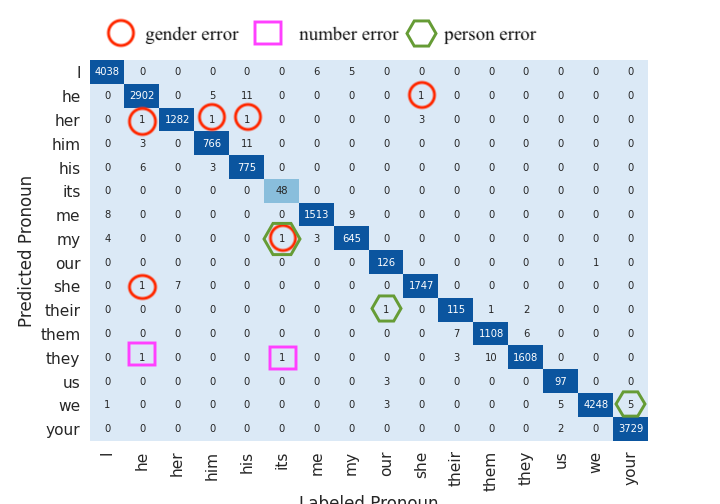
\includegraphics[scale = 0.55]{circle.png}
    \caption{The Non-case Errors produced by \texttt{aX + Xb} model}
    \label{fig:circle}
\end{figure}
\FloatBarrier



\subsection{Conclusion}
This section explored the possibility of using distribution patterns to distinguish pronoun cases. Models on the fixed trigram frame \texttt{aXb} and flexible frame \texttt{aX + Xb} with a large sample size and a smaller one were trained. The results showed that the distributional patterns are extremely effective in categorizing grammatical case of pronouns. Based on the high accuracy results with case categorization, this study further explored pronoun categorization with person, gender, and number information as additional input. With large sample size, the model achieved almost perfect pronoun categorization accuracy. The experiments showed that distributional patterns in parents' input are very useful in categorizing grammatical cases. The model showed a similar accuracy rate as children's real-life pronoun case acquisition. However, the similar accuracy rate does not demonstrate that children actually utilize distributional patterns in learning and the differences between the errors made by training models and by children suggest children may be using a different procedure or an additional procedure. Further investigations of the classification errors and children's pronoun case errors will be informative for understanding the process of case categorization. 

